\vspace{5pt}\\\scalebox{0.6}{
\begin{minipage}{\textwidth}
\centering
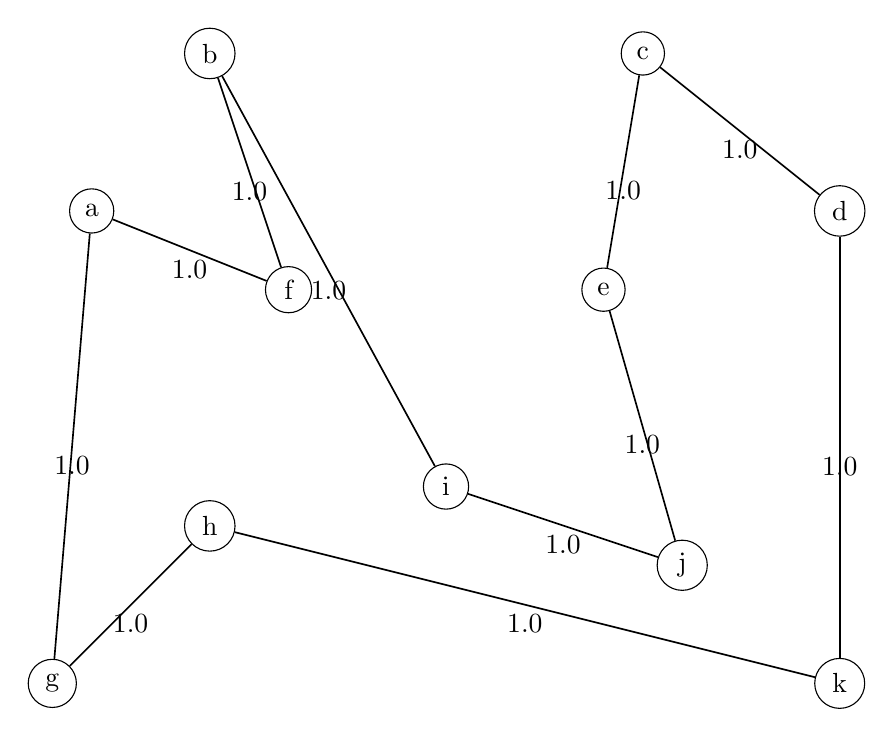
\begin{tikzpicture}
\begin{scope}[every node/.style = {circle, draw}]
\node (a) at (0.5, 6) {a};
\node (b) at (2, 8) {b};
\node (c) at (7.5, 8) {c};
\node (d) at (10, 6) {d};
\node (e) at (7, 5) {e};
\node (f) at (3, 5) {f};
\node (g) at (0, 0) {g};
\node (h) at (2, 2) {h};
\node (i) at (5, 2.5) {i};
\node (j) at (8, 1.5) {j};
\node (k) at (10, 0) {k};
\end{scope}
\begin{scope}[every edge/.style = {draw, semithick}]
\path (a) edge node[anchor=north] {1.0} (f);
\path (a) edge node[anchor=north] {1.0} (g);
\path (b) edge node[anchor=north] {1.0} (f);
\path (b) edge node[anchor=north] {1.0} (i);
\path (c) edge node[anchor=north] {1.0} (d);
\path (c) edge node[anchor=north] {1.0} (e);
\path (d) edge node[anchor=north] {1.0} (k);
\path (e) edge node[anchor=north] {1.0} (j);
\path (g) edge node[anchor=north] {1.0} (h);
\path (h) edge node[anchor=north] {1.0} (k);
\path (i) edge node[anchor=north] {1.0} (j);
\end{scope}
\end{tikzpicture}
\end{minipage}
}\vspace{5pt}\\
